
The equation of curve can be expressed as 
\begin{align}
  y+\frac{2}{x-3}=0  \\
  xy-3y+2=0\label{quadform/41/eq:giveneq}
\end{align}
Comparing with the standard equation, 
\begin{align}
\vec{x}^T\vec{V}\vec{x}+2\vec{u}^T\vec{x}+f=0\\
\vec{V}=\myvec{0&\frac{1}{2}\\\frac{1}{2}&0},\vec{u}=\myvec{0\\-\frac{3}{2}},f=2\\
\vec{V}^{-1}=\myvec{0&2\\2&0}
\end{align}
$\because$
\begin{align}
    \abs{\vec{V}} &= \frac{-1}{4}
    \\
    \implies \abs{\vec{V}} &< 0
\end{align}
and \eqref{quadform/41/eq:giveneq} represents a hyperbola.
The characteristic equation of $\vec{V}$ is 
\begin{align}
    \abs{\vec{V} - \lambda\vec{I}} = \mydet{-\lambda & \frac{1}{2} \\ \frac{1}{2} & -\lambda} &= 0
    \\
    \implies \lambda^2 - \frac{1}{4} &= 0
\end{align}
and the eigenvalues are 
\begin{align}
    \lambda_1 = \frac{1}{2} , \lambda_2 = \frac{-1}{2}
\end{align}
% Eigen vector $\vec{p}$ is 
% \begin{align}
%     \vec{V}\vec{p} &= \lambda\vec{p}
%     \\
%     \implies (\vec{V} - \lambda\vec{I})\vec{p} &= 0
% \end{align}
Eigen vector $\vec{p}_1$ corressponding to $\lambda_1$ can be obtained as
\begin{align}
    (\vec{V} - \lambda_1\vec{I}) &= \myvec{\frac{-1}{2} & \frac{1}{2} \\ \frac{1}{2} & \frac{-1}{2}}\xleftrightarrow[R_1 \leftarrow -2R_1]{R_2 = R_1 + R_2}\myvec{1 & -1 \\ 0 & 0}
    \\
    \implies \vec{p_1} &= \frac{1}{\sqrt{2}}\myvec{1 \\ 1}
\end{align}
Similarly,
\begin{align}
    \vec{p_2} &= \frac{1}{\sqrt{2}}\myvec{-1 \\ 1}
\end{align}
$\therefore$
\begin{align}
    \vec{P} &= \myvec{\vec{p_1} & \vec{p_2}} = \frac{1}{\sqrt{2}}\myvec{1 & -1 \\ 1 & 1}
    \\
    \vec{D} &= \myvec{\lambda_1 & 0 \\ 0 & \lambda_2} = \myvec{\frac{1}{2} & 0 \\ 0 & \frac{-1}{2}}
\end{align}
Now,
\begin{align}
    \vec{c} &= -\vec{V}^{-1}\vec{u} 
    \\
    &= -\myvec{0 & 2 \\2 & 0}\myvec{0 \\ \frac{-3}{2}}
    \\
    &= \myvec{3 \\ 0}
\end{align}
\begin{align}
\because \vec{u}^T\vec{V}^{-1}\vec{u} - f<0,
\end{align}
the axes need to be swapped and 
\begin{align}
    \sqrt{\frac{ \vec{u}^T\vec{V}^{-1}\vec{u} - f}{\lambda_2}} &= 2
    \\
    \sqrt{ \frac{f- \vec{u}^T\vec{V}^{-1}\vec{u}}{\lambda_1}} &= 2
\end{align}
$\therefore$ the equation of the standard hyperbola can be expressed as 
\begin{align}
    \frac{y^2}{4} - \frac{x^2}{4} &= 1
\end{align}
The direction and normal vectors of tangent with slope 2 are 
\begin{align}
    \vec{m}=\myvec{1\\2},\vec{n}=\myvec{-2\\1}
\end{align}
From the  conics table in the manual,
\begin{align}
\kappa = \pm \sqrt{\frac{\vec{u}^T\vec{V}^{-1}\vec{u}-f}{\vec{n}^T\vec{V}^{-1}\vec{n}}} = \pm \sqrt{\frac{1}{4}} = \pm \frac{1}{2}
\end{align}
and the desired points of contact are 
\begin{align}
\vec{q}&=\vec{V}^{-1}(\kappa\vec{n}-\vec{u})\\
\implies \vec{q}_1=\myvec{4\\-2}, 
\vec{q}_2=\myvec{2\\2}\label{quadform/41/eq:10}
\end{align}
The equation of the tangents are given by
\begin{align}
    \vec{n}^T\vec{x}&=\vec{n}^T\vec{q}\\
    \implies \myvec{-2&1}\vec{x}&=\myvec{-2&1}\myvec{4\\-2}=-10\\
    \text{and }\myvec{-2&1}\vec{x}&=\myvec{-2&1}\myvec{2\\2}=-2
\end{align}
%
The above results are verified in Fig. \ref{quadform/41/fig:tangents}.	
\begin{figure}[!ht]
\centering
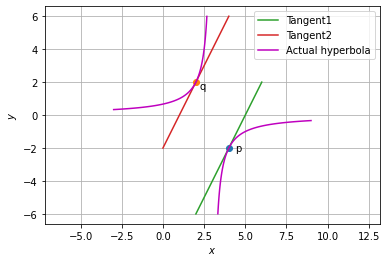
\includegraphics[width=\columnwidth]{solutions/su2021/2/41/figure6_1.png}
\caption{The tangents to the curve with slope 2 }
\label{quadform/41/fig:tangents}	
\end{figure}

